\documentclass[11pt,conference]{IEEEtran}

\ifCLASSINFOpdf
   \usepackage[pdftex]{graphicx}
  % declare the path(s) where your graphic files are
   \graphicspath{{../pdf/}{../jpeg/}}
  % and their extensions so you won't have to specify these with
  % every instance of \includegraphics
   \DeclareGraphicsExtensions{.pdf,.jpeg,.png}
\else
  % or other class option (dvipsone, dvipdf, if not using dvips). graphicx
  % will default to the driver specified in the system graphics.cfg if no
  % driver is specified.
  \usepackage[dvips]{graphicx}
  % declare the path(s) where your graphic files are
  \graphicspath{{../eps/}}
  % and their extensions so you won't have to specify these with
  % every instance of \includegraphics
  \DeclareGraphicsExtensions{.eps}
\fi


\usepackage[utf8x]{inputenc}
\usepackage[T1]{fontenc}
\usepackage{lmodern}
\usepackage{booktabs}
\usepackage{multirow}
\usepackage{algorithmic}
\usepackage[Algoritmo]{algorithm}
\usepackage[spanish,USenglish]{babel}
\usepackage[colorlinks=true,linkcolor=black,urlcolor=black,citecolor=black, urlcolor=black, filecolor=black bookmarks=false]{hyperref}
\usepackage{subfigure}
\usepackage{array}
\usepackage{color}
\usepackage{graphicx}
\usepackage{epsfig}
\usepackage{multirow}
\usepackage{colortbl}
\usepackage[table]{xcolor}

\addto\captionsspanish{
 \def\tablename{Tabla}}


\begin{document}

\pagestyle{empty}  

\selectlanguage{spanish}

\title{Informe trabajo práctico número dos - Aprendizaje Automático}

\author{\IEEEauthorblockN{Omar Ernesto Cabrera Rosero}
\IEEEauthorblockA{Universidad de Buenos Aires\\
%Buenos Aires, Argentina\\
Email: omarcabrera@udenar.edu.co}
\and
\IEEEauthorblockN{Jimmy Mateo Guerrero Restrepo}
\IEEEauthorblockA{Universidad de Buenos Aires\\
%Buenos Aires, Argentina\\
Email: jimaguere@gmail.com}
}

\maketitle

%\selectlanguage{USenglish}
\begin{abstract}

En este trabajo pŕactico se desarrolla un modelo de predicción del rango del precio de $m^2$ de propiedades
a la venta en la Ciudad de Buenos Aires, de esta forma poder estimar el rango del precio del $m^2$ de un inmueble para
decidir el nivel de especialista que se destinará para realizar la inspección física y así obtener una cotización real
del precio en venta. Para la realización del modelo se tuvo en cuenta conceptos de árboles de decisión, resamplig,
ensamble y minería de texto.

\end{abstract}
 
\selectlanguage{spanish}


\begin{IEEEkeywords}
Árboles de decisión, clasificación, inmobiliaria, resampling, ensamble, minería de texto.
\end{IEEEkeywords}

\thispagestyle{empty} 

\IEEEpeerreviewmaketitle

\section{Introducción}

La Inmobiliaria www.barealestate.com.ar dispone de un sitio Web para la compra y
venta de inmuebles en la Ciudad de Buenos Aires. Para disminuir los costos de
publicación, necesita disponer de una pre-valorización de los inmuebles publicados a la
venta por los propietarios.

La empresa necesitaría de alguna forma estimar el rango del precio del metro cuadrado del
inmueble para decidir el nivel de especialista que destinará para realizar una
inspección física y así obtener una cotización real del precio de venta. Para la
empresa, el costo de la publicación depende mucho del nivel del especialista que tiene
que realizar la cotización, por lo tanto, desea bajarlo manteniendo acotado el riesgo de
una mala cotización.

Se usaron dos conjuntos de datos, uno para entrenamiento con 15.000 registros y otro con 4.000 registros para devolverlo clasificado, 
el conjunto de datos tiene 5 clases las cuales vienen dadas de la siguiente manera:

\begin{itemize}
 \item Clase 1: $m^2$ <= \$2.000
 \item Clase 2: \$2.000 < $m^2$ <= \$2.500
 \item Clase 3: \$2.500 < $m^2$ <= \$5.500
 \item Clase 4: \$5.500 < $m^2$ <= \$18.500
 \item Clase 5: \$18.500 < $m^2$
\end{itemize}

El objetivo de este trabajo práctico es desarrollar un modelo de predicción del rango
del precio del metro cuadrado de propiedades a la venta en la Ciudad de Buenos Aires, realizando
modelos de predicción teniendo en cuenta conceptos de árboles de decisión, minería de texto,
resampling y ensamble.
\section{Metodología}

Se utilizó la metodología CRISP-DM (Cross Industry Standard Process for Data Mining) uno
de los modelos principalmente utilizados en los ambientes académico e industrial y la
guía de referencia más ampliamente utilizada \cite{hernandez2004}.

Esta metodología contempla seis fases: entendimiento del negocio, entendimiento
de los datos, preparación de los datos, modelado, evaluación e implementación, que se
describen a continuación.

\subsection{Entendimiento del Negocio}

Se adquirió conocimiento en cuanto a la valorización en metros cuadrados, teniendo en cuenta factores como lo son
la ubicación, cantidad de ambientes, superficie total, piso en el que se encuentra el departamento y hacer un análisis de
minería de texto en las descripciones que tienen cada departamento.

\subsection{Entendimiento de los Datos}
Se construyó un conjunto de datos y se analizó cada atributo, realizando un análisis exploratorio de datos como por ejemplo
tabla de frecuencias, datos nulos e identificadores únicos.

Se puede observar la frecuencias de las palabras en la figura~\ref{fig:tf}.

\begin{figure}
  \centering
  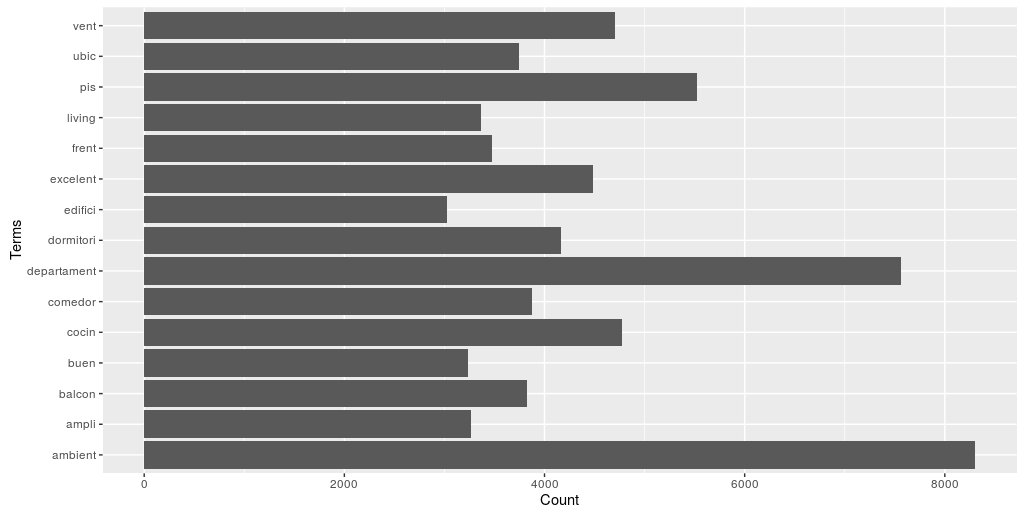
\includegraphics[width = 9cm]{tabla_frecuencias_texto.png}
  \caption{Frecuencias de palabras}
  \label{fig:tf}
\end{figure}

\subsection{Preparación de los Datos}
La preparación de datos para construir el conjuntos de datos de entrenamiento se lo realizó teniendo en cuenta las
siguientes transformaciones:

\begin{itemize}
 \item Se aplico minería de texto al atributo lugar de tal manera que se hizo el cambio del nombre del barrio a columnas
 debido a que los algoritmos implementados como random forest únicamente admiten un máximo de 53 categorías en cada atributo
 y no admite datos nulos.
 
 \item Para evitar los datos nulos se utilizo estrategias de relleno: tanto a los pisos como los ambientes que tenían datos nulos 
 se los relleno con el valor de ``1'', para la superficie total de metros cuadrados que estaban nulos se el asignó la superficie cubierta
 de metros cuadrados, este mismo proceso se lo realizó luego en sentido contrario.
 
 \item Se eliminaron las siguientes columnas: ident, fecha, geoname\_num, lat\_lon.
 
 \item Se fusionó los textos de las columnas des y tit, y luego se les aplico minería de texto, además se hizo una limpieza
 de acentos, palabra muertas, se removió los números y espacios en blanco.
 
 \item Antes de aplicar las técnicas de modelado, se procedió a
evaluar la calidad y relevancia de los atributos del conjunto de datos
 con el objetivo de predecir valores de la clase buscada. Se
utilizó el algoritmo ``boruta'' propuesto en \cite{kursa2010feature} para la extracción y
evaluación de atributos. El algoritmo está diseñado como un recubrimiento alrededor del algoritmo de clasificación random
forest y califica cada atributo en el conjunto de datos de
acuerdo a su importancia a la hora de clasificar. Se puede observar la relevancia en la nube de palabras que se muestra
en la figura~\ref{fig:np} 
\end{itemize}

\begin{figure}
  \centering
  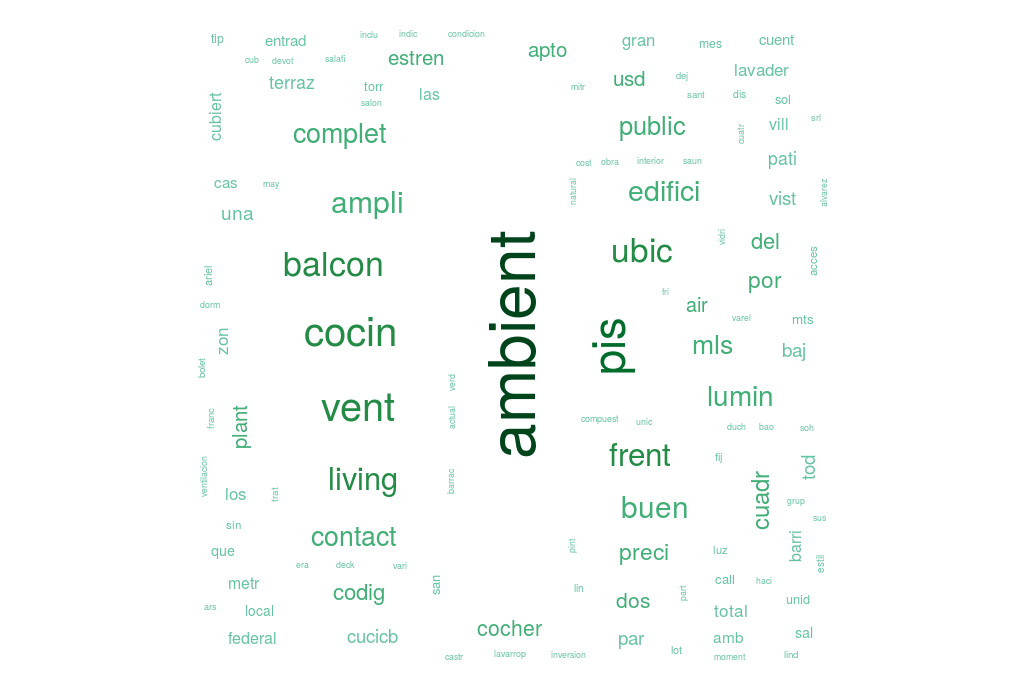
\includegraphics[width = 11cm]{words.png}
  \caption{Nube de palabras}
  \label{fig:np}
\end{figure}

Teniendo en cuenta las anteriores transformaciones descritas se crearon varios conjuntos de 
datos para luego poder aplicarles modelos de clasificación, la tabla~\ref{table:conjunto} muestra
el conjunto de datos, con su descripción, el nombre del conjunto viene representado con una ``V'' que
es el número de variables y una ``R'' para el número de registro del conjunto. 

Los conjuntos de datos se los puede descargar desde el repositorio\footnote{\url{https://github.com/poldrosky/tp2AA}}. 


\begin{table}
\begin{center}
\caption{Conjuntos de Datos}
\label{table:conjunto}
\begin{tabular}{|c|c|}
\hline
  \rowcolor{blue!55} 
   \multicolumn{1}{|c|}{Nombre del conjunto} & \multicolumn{1}{c|}{Descripción} \\ \hline
    & Variables propias del conjunto. \\
        & Minería de texto a la descripción. \\
        & Minería de texto al lugar. \\
   V1797R9714 & Aplicación de algoritmo boruta al lugar. \\
        & Frecuencia de texto mayor a 10. \\ 
        & Sin estrategia de relleno. \\
        & Eliminación de registros nulos. \\ \hline
      &   Variables propias del conjunto.\\
        & Mineria de texto al lugar. \\
   V81R9714 & No se usó la descripción. \\
        & Sin estrategia de relleno. \\
        & Eliminación de registros nulos. \\ \hline
    & Variables propias del conjunto.\\
        & Mineria de texto al lugar. \\
   V57R9714 & Aplicación de algoritmo boruta al lugar. \\
        & No se usó la descripción. \\
        & Sin estrategia de relleno. \\
        & Eliminación de registros nulos. \\ \hline
        & Se rellenaron datos faltantes. \\
   V3385R14625 & Variables propias del conjunto. \\
	& Minería de texto a la descripción. \\
        & Frecuencia de texto mayor a 3. \\
        & Minería de texto al lugar. \\ \hline
        & Se rellenaron datos faltantes. \\ 
        & Variables propias del conjunto. \\
   V2652R14625 & Minería de texto al lugar. \\
        & Minería de texto a la descripción. \\
        & Frecuencia de texto mayor a 5. \\ \hline
        & Se rellenaron datos faltantes. \\ 
        & Variables propias del conjunto. \\
   V221R14625 & Minería de texto a la descripción. \\
        & Frecuencia de texto mayor a 5. \\
        & Minería de texto al lugar. \\
        & Aplicación de algoritmo boruta. \\ \hline
    \end{tabular}
\end{center}
\end{table}



\subsection{Modelado}

Para la etapa de modelado se utilizó el modelo de predicción random forest, el cual se basa en el desarrollo de
muchos árboles de clasificación. Para clasificar un nuevo objeto desde un vector de entrada,
ponemos dicho vector bajo cada uno de los árboles generados. Cada árbol tiene una clasificación, 
en términos coloquiales diríamos que cada árbol  selecciona una clase. Finalmente se escoge 
la clasificación teniendo en cuenta el árbol más votado sobre todos los demás. 

En la tabla~\ref{table:performance} se muestra los resultados al aplicar random forest en los conjuntos
generados en la etapa de preparación de datos.

\begin{table}
\begin{center}
\caption{Performance de los conjuntos}
\label{table:performance}
\begin{tabular}{|c|c|}
\hline
  \rowcolor{blue!55} 
   Nombre del conjunto & Performance \\ \hline
   V1797R9714 & 0.533 \\ \hline
   V81R9714 & 0.455 \\ \hline
   V57R9714 & 0.466 \\ \hline
   V3385R14625 & 0.529 \\ \hline
   V2652R14625 & 0.528 \\ \hline
   V221R14625 & 0.549 \\ \hline
    \end{tabular}
\end{center}
\end{table}

El conjunto de datos que tiene la mejor performance es ``V221R14625'' el cual esta compuesto
por 221 variables y 14525 registros, a este conjunto se le aplicaron otros modelos y se evaluo la performance, los 
resultados se pueden ver en la tabla~\ref{table:performanceV221R14625}.

Estos modelos fueron creados utilizando la biblioteca de código abierto rminer presentada por \cite{cortez2010data} para la
herramienta R.

\begin{table}
\begin{center}
\caption{Performance conjunto V221R14625}
\label{table:performanceV221R14625}
\begin{tabular}{|c|c|}
\hline
  \rowcolor{blue!55} 
   Modelos & Performance \\ \hline
   ctree & 0.435 \\ \hline
   rpart & 0.391 \\ \hline
   kknn & 0.425 \\ \hline
   ksvm & 0.471 \\ \hline
   random forest & 0.549 \\ \hline
   bagging & 0.384 \\ \hline
   lda & 0.436 \\ \hline
   naiveBayes & 0.351 \\ \hline
 \end{tabular}
\end{center}
\end{table}

\subsection{Evaluación} 

Se evaluaron clasificadores tanto como arboles de decisión, como modelos probalísticos. El mejor árbol
que tubo mejor perfonmance fue el árbol de decisión ``random forest'', y el modelo probabilístico
que tubo mejor perfomance fue el modelo ``linear discriminant analysis (lda)''.

\subsection{Implementación} 

La etapa de implementación se la realizo utilizando resampling y ensamble para luego
aplicarse en el conjunto de prueba. 

Para el ensamble se hizo resampling con el conjunto de datos de 221 variables,
con el cual se tenia un 54\% de performance. El conjunto de datos  se partió por filas (resampling por filas)  en 4 partes
aleatorias, cada una con el 25\% del total filas, a cada partición se les aplico modelos  random forest variando los parámetros
del algoritmo. 

Una vez generados los cuatro modelos de clasificación se tomo el conjunto a clasificar
y se realizaron las predicciones con dichos modelos. Para generar el conjunto de datos de clasificación se realizo una votación simple
con los resultados predichos por los cuatro modelos. Para los casos en que alguno de 
los modelos no arrojaba una clasificación o había un empate de clases entre los 
modelos, se utilizo  el modelo ``lda'' para clasificar las instancia no clasificadas o para desempatar la decisión.
 
\section{Conclusiones}

Se construyón un modelo de clasificación para resolver el problema para predecir el precio del $m^2$  
a la venta en la Ciudad de Buenos Aires, de esta forma poder estimar el rango del precio del $m^2$ de un inmueble.

El árbol random forest, resultó ser el mejor clasificador de árboles debido a que se basa en el desarrollo de
muchos árboles de clasificación que dependen de un vector aleatorio probado independientemente y con la 
misma distribución para cada uno de estos.

El hacer resampling por filas sirve para generar varios modelos, y con ellos realizar votación, esto ayuda
a que al aplicar estos modelos, se pueda hacer una votación y se pueda quedar con el que valor con más frecuencia.

Cuando se aplica árboles de decisión algunos datos no se van a clasificar, por esta razón fue necesario utilizar
un clasificador probabilístico para los datos que no fueron clasificados.




%\appendices
%\section{Repositorio}
%El código fuente y conjunto de datos se encuentran en el repositorio de github.



% Can use something like this to put references on a page
% by themselves when using endfloat and the captionsoff option.
\ifCLASSOPTIONcaptionsoff
  \newpage
\fi


\bibliographystyle{IEEEtran}

\bibliography{IEEEabrv,bibliography}



\end{document}
